\section{Implementation}
\label{passert:sec:implementation}

We implemented \tool using the LLVM compiler infrastructure~\cite{llvm}. \tool
compiles source programs written in C and C++ to the LLVM intermediate
language, probabilistically evaluates the resulting bitcode programs by extracting
probability distributions, optimizes the resulting distributions, and
then evaluates the \passert distributions either exactly or with sampling.

\paragraph{Language and Interface}

To use \tool, the programmer adds a \passert to her program and annotates
certain functions as probability distributions or uses a provided library of
common distributions. Both constructs are implemented as C macros provided by
a \texttt{passert.h} header: \texttt{PASSERT(e)} marks an expression that
\tool will evaluate and \texttt{DISTRIBUTION} marks functions
that should be treated as a symbolic probability distribution.

The programmer invokes \tool and provides the source files and command-line
arguments for the execution along with optional $\alpha$ and $\epsilon$ values
that control confidence and accuracy. \tool reports a confidence interval on
the output probability and the results of the hypothesis test (true, false, or
unverifiable).

\paragraph{Distribution Extraction}

The distribution extraction analysis is implemented as an instrumented
interpreter of LLVM bitcode programs. \tool maintains a symbolic heap and
stack. Each symbolic value is a pointer into an object graph representing a
Bayesian network. Nodes in the graph correspond to the expression tree language of
our formalism: they can be samples, arithmetic operations, comparisons,
constants, or conditionals.

The implementation conserves space by coalescing identical expression trees.
For example, consider the values
$e_1 = \{ s_1 + s_2 \}$ and $e_2 = \{ (s_1 + s_2) + s_3 \}$ consisting of sums of samples.
In a naive implementation of probabilistic evaluation, these would be independent trees
that refer to a global set of samples at their leaves.
Instead, \tool implements $e_2$ as a sum node with two
children, one of which is the node for $e_1$.
In this sense, \tool maintains a global Bayesian network for the
execution in which
values are pointers into the network.

Nodes in the Bayesian network can become unreachable when heap values are
overwritten and as stack frames are popped.
\tool reclaims memory in these cases by reference-counting all nodes in the
Bayesian network.
The root set consists of stack and heap values.
Since Bayesian networks are acyclic, reference counting is sufficient.

When operating on non-probabilistic values (e.g., when evaluating $1 + 2$),
\tool avoids constructing nodes in the Bayesian network and instead maintains
a concrete heap and stack. We use the
bitcode interpreter that ships with LLVM~\cite{llvminterp} to perform
the concrete operations.
This process can be viewed as an optimization on Bayesian networks for
operations over point-mass distributions.

\edef\optsdata#1{%
\ifstrequal{#1}{gpswalk-arithIdent}{1914}{}%
\ifstrequal{#1}{gpswalk-clt}{1}{}%
\ifstrequal{#1}{gpswalk-knownDist}{0}{}%
\ifstrequal{#1}{hotspot-arithIdent}{1}{}%
\ifstrequal{#1}{hotspot-clt}{1}{}%
\ifstrequal{#1}{hotspot-knownDist}{24064}{}%
\ifstrequal{#1}{inversek2j-arithIdent}{901}{}%
\ifstrequal{#1}{inversek2j-clt}{1}{}%
\ifstrequal{#1}{inversek2j-knownDist}{200}{}%
\ifstrequal{#1}{kmeans-arithIdent}{2149}{}%
\ifstrequal{#1}{kmeans-clt}{0}{}%
\ifstrequal{#1}{kmeans-knownDist}{300}{}%
\ifstrequal{#1}{salary-abs-arithIdent}{5003}{}%
\ifstrequal{#1}{salary-abs-clt}{1}{}%
\ifstrequal{#1}{salary-abs-knownDist}{1}{}%
\ifstrequal{#1}{salary-arithIdent}{3}{}%
\ifstrequal{#1}{salary-clt}{1}{}%
\ifstrequal{#1}{salary-knownDist}{1}{}%
\ifstrequal{#1}{sobel-arithIdent}{7880}{}%
\ifstrequal{#1}{sobel-clt}{1}{}%
\ifstrequal{#1}{sobel-knownDist}{0}{}%
}


\begin{sidewaystable}
    \centering
    \small
    \begin{tabular}{l
    >{\raggedright\arraybackslash} p{2.7in}
    r r r
    r r r}
        \toprule
        &&\multicolumn{3}{c}{Time (seconds)}
        &\multicolumn{3}{c}{Optimization Counts}
        \\ \cmidrule(lr){3-5} \cmidrule(lr){6-8}
        Program &
        Description and \passert &
        Baseline &
        Analysis &
        Sampling &
        Arith &
        Dist Op &
        CLT
        \\
        \midrule
        \bench{gpswalk} &
Location sensing and velocity calculation \newline
\passert: Velocity is within normal walking speed &
\perfdata{time-gpswalk-dummy-run} &
\perfdata{time-gpswalk-sample-analyze} &
\perfdata{time-gpswalk-sample-run} &
\optsdata{gpswalk-arithIdent} &
\optsdata{gpswalk-knownDist} &
\optsdata{gpswalk-clt}
\\
\addlinespace[0.6ex]
\bench{salary} &
Calculate average of concrete obfuscated salaries \newline
\passert: Obfuscated mean is close to true mean &
\perfdata{time-salary-dummy-run} &
\perfdata{time-salary-sample-analyze} &
\perfdata{time-salary-sample-run} &
\optsdata{salary-arithIdent} &
\optsdata{salary-knownDist} &
\optsdata{salary-clt}
\\
\addlinespace[0.6ex]
\bench{salary-abs} &
\bench{salary} with abstract salaries drawn from a distribution \newline
\passert: As above &
\perfdata{time-salary-abs-dummy-run} &
\perfdata{time-salary-abs-sample-analyze} &
\perfdata{time-salary-abs-sample-run} &
\optsdata{salary-abs-arithIdent} &
\optsdata{salary-abs-knownDist} &
\optsdata{salary-abs-clt}
\\
\addlinespace[0.6ex]
\bench{kmeans} &
Approximate clustering \newline
\passert: Total distance is within threshold &
\perfdata{time-kmeans-dummy-run} &
\perfdata{time-kmeans-sample-analyze} &
\perfdata{time-kmeans-sample-run} &
\optsdata{kmeans-arithIdent} &
\optsdata{kmeans-knownDist} &
\optsdata{kmeans-clt}
\\
\addlinespace[0.6ex]
\bench{sobel} &
Approximate image filter \newline
\passert: Average pixel difference is small &
\perfdata{time-sobel-dummy-run} &
\perfdata{time-sobel-sample-analyze} &
\perfdata{time-sobel-sample-run} &
\optsdata{sobel-arithIdent} &
\optsdata{sobel-knownDist} &
\optsdata{sobel-clt}
\\
\addlinespace[0.6ex]
\bench{hotspot} &
Approximate CMOS thermal simulation \newline
\passert: Temperature error is low &
\perfdata{time-hotspot-dummy-run} &
\perfdata{time-hotspot-sample-analyze} &
\perfdata{time-hotspot-sample-run} &
\optsdata{hotspot-arithIdent} &
\optsdata{hotspot-knownDist} &
\optsdata{hotspot-clt}
\\
\addlinespace[0.6ex]
\bench{inversek2j} &
Approximate robotics control \newline
\passert: Computed angles are close to inputs &
\perfdata{time-inversek2j-dummy-run} &
\perfdata{time-inversek2j-sample-analyze} &
\perfdata{time-inversek2j-sample-run} &
\optsdata{inversek2j-arithIdent} &
\optsdata{inversek2j-knownDist} &
\optsdata{inversek2j-clt}
\\

        \bottomrule
    \end{tabular}
    \caption{
        Programs used in the evaluation.
        The \passert for each application describes a probabilistic
        correctness property.
        The \emph{time} columns indicate the time taken by the baseline
        stress-testing strategy, \tool's analysis, and \tool's sampling step.
        The \emph{optimization counts} reflect the three categories of
        optimizations applied by \tool: arithmetic identities (Arith), operations on
        known closed-form distributions (Dist Op), and the Central Limit
        Theorem optimization (CLT).
    }
    \label{passert:table:apps}
\end{sidewaystable}

\paragraph{Conditionals}

Conditionals appear as branches in LLVM IR.
\tool analyzes conditionals by
symbolically executing both sides of the branch and merging the resulting heap
updates. When the analysis encounters a branch, it finds the immediate post-dominator
(ipdom) in the control-flow graph---intuitively, the join point---and begins by taking
the branch. In this phase, it buffers all heap writes in a (scoped) hash table.
Then, when the ipdom is reached, control returns to the
branch and follows the not-taken direction.
Writes in this phase do not go into the scope for the current conditional:
they propagate to the global heap or, if execution is in a nested outer
conditional, to the enclosing hash table scope.
When the ipdom is reached the second time, the buffered writes are
merged into the outer heap using conditional nodes.

\paragraph{Probabilistic Pointers}

\tool adds limited support for symbolic pointers for probabilistic array
indexing. Programs can load and store from \code{arr[i]} where \code{i} is
probabilistic, which \tool handles with a probabilistic extension of the
theory of
arrays. Pointers and array indices must be finite discrete
distributions so we can enumerate the set of locations to which a pointer $p$
might refer, i.e., those addresses where $p$'s distribution has non-zero
probability.
Loading from a symbolic pointer $p$ yields a distribution that
reflects the set of values at each such location, while storing to
$p$ updates each location to compose its old and new value
under a conditional distribution.

\paragraph{Bayesian Network Optimizations}

\tool performs statistical optimizations as transformations on the Bayesian
network representation as outlined in Section~\ref{passert:sec:optim}. The
optimizations we implemented fall into three broad categories,
which we characterize empirically in the next section.

The first category consists of arithmetic identities, including
binary operators on constants, comparisons with extremes (e.g.,
C's \code{FLT_MAX}), and addition or multiplication with a constant zero.
These optimizations do not exploit the probabilistic properties of the
Bayesian network but compose with more sophisticated optimizations and enhance
the tool's partial-evaluation effect.
The next category consists of operations on known probability distributions,
including the addition of two normal distributions, addition or
multiplication with a scalar, comparison between distributions with disjoint
support, comparison between two uniform distributions, and comparison with a
scalar (i.e., CDF queries).
These optimizations exploit our probabilistic view of the program to apply
well-known statistical properties of common distributions.
The final optimization we evaluate is the Central Limit Theorem, which
collapses a summation of distributions into a single normal.

Some optimizations, such as basic arithmetic identities, are performed
opportunistically on-the-fly during analysis to reduce \tool's memory
footprint.
Others, such as the Central Limit Theorem transformation, operate only on the
complete graph.
Internally, the on-line optimizer also collapses deep trees of commutative
arithmetic operators into ``fat'' sum and product nodes with many children.
This rewriting helps the optimizer identify constants that can be coalesced and
inverse nodes that cancel each other out.



\paragraph{Verification via Direct Evaluation or Sampling}
As described in Section~\ref{passert:sec:verification}, the prior
optimizations often produce Bayesian networks that \tool can
directly evaluate.  In other cases, \tool must sample the
optimized Bayesian network, in which case \tool generates LLVM bitcode
that samples from the Bayesian network.
The tool then compiles the generated program to machine code and executes
it repeatedly to perform statistical verification.


%%%%%%%%%%%%%%%%%%%%%%%%%%%%%%%%%%%%%%%%%%%%%%%%%%%%%%%%%%%%%%%%%%%%%%%%

\section{Evaluation}
\label{passert:sec:evaluation}


This section describes our experience expressing \passerts in a variety of
probabilistic programs and using \tool to verify them.

\subsection{Benchmarks}

We evaluate \passerts in five probabilistic programs
from three domains: sensors, differential privacy, and approximate
computing. 
Table~\ref{passert:table:apps} summarizes the set of programs and the \passert
statements we added to each.

Programs that compute with noisy sensor data, such as GPS,
accelerometers, and video game motion sensors, behave
probabilistically~\cite{PPT:05,uncertaint}. To demonstrate our
approach on this class of applications, we implemented a common
mobile-phone application: estimating walking speed~\cite{uncertaint}.
\bench{gpswalk} processes a series of noisy coordinate readings from a mobile
phone and computes the walking speed after each reading.
The GPS error follows a Rayleigh distribution and is determined by the sensor's
uncertainty estimate.
As Bornholt et al.~\cite{uncertaint} note, this kind of sensing workload can
produce wild results when an individual location reading is wrong.
The \passert checks that the computed velocity is below a maximum walking
speed.

Differential privacy obfuscates personal data at the cost of
accuracy~\cite{pinq, airavat, gupt, fuzz, certipriv}.
To study how \tool works on this class of application, we
implemented two benchmarks.
\bench{salary} reads a list of 5000 salaries of Washington state public
employees
and computes their average.\footnote{Source: \url{http://fiscal.wa.gov/}}
The program obfuscates each salary by adding a normal distribution ($\sigma^2
= 3000$) to simulate a situation where each employee is unwilling to divulge
his or her exact salary. The \passert checks whether the obfuscated average is
within 25 dollars of the true average.
We also evaluate a version of the program, \bench{salary-abs}, where the input
salaries are drawn from a uniform distribution instead of read from a file.
This variant highlights a scenario where specific inputs are unavailable and
we instead want to check a \passert given an input probability distribution.

The final class of applications is drawn from prior work on
approximate computing: \bench{kmeans}, \bench{sobel}, \bench{hotspot}, and
\bench{inversek2j} represent programs
running on approximate hardware~\cite{truffle, pcmos, stochasticproc}.
\bench{sobel} implements the Sobel filter, an image convolution used in edge
detection.
\bench{kmeans} is a clustering algorithm.
\bench{hotspot} simulates thermal activity on a microprocessor. \bench{inversek2j} uses inverse kinematics to compute a robotic arm's
joint angles given a target position.
Both \bench{kmeans} and \bench{hotspot} are drawn from the Rodinia 2.4
benchmark suite~\cite{rodinia} while \bench{sobel} and \bench{inversek2j} are
approximate applications from Esmaeilzadeh et al.~\cite{npu}.
In all cases, we add random calls that
simulate approximate arithmetic operations on inner computations.
The \passert bounds the error of the program's overall output.
For most benchmarks, the error is measured with respect to the output of a
precise version of the computation, but in \bench{inversek2j}, we use the
corresponding forward kinematics algorithm to check the result.

For both approximate and data privacy programs, we compare a
precise version of a function's output with a perturbed version.
In the sensing workload, \bench{gpswalk}, the data is intrinsically noisy, so
there is no ``ground truth'' to compare against.
For the
purposes of this evaluation, we manually extended the programs to compute both
results. A simple ``desugaring'' step could help perform this transformation
automatically by duplicating the code, removing randomization from one
copy, and returning both results.

\subsection{Performance}

To evaluate \tool's performance benefits,
we compare its total running time against
using a simple stress testing baseline.
The baseline checker adds a \code{for} loop around the entire
probabilistic program and counts the number of times the \passert expression
is true.
The time taken for a \tool verification includes the time to extract and
optimize a probability distribution and to repeatedly sample the
result.
We test all programs with a confidence of $\alpha = 0.05$ and an
accuracy of $\epsilon = 0.01$, which leads to 74147 samples.
(Recall from Section~\ref{passert:sec:sample} that the sample count depends only on the
$\alpha$ and $\epsilon$ parameters and 
 so we sample all programs the
same number of times.)
Table~\ref{passert:table:apps} lists the absolute running times and
Figure~\ref{passert:fig:performance} visualizes the normalized performance.
The timings are averaged over 5 executions collected on a dual-core 2~GHz
Intel Core 2 Duo with 4~GB of memory.
On average, \tool verification takes \perfdata{o-normtime-harmmean-sample} as
long as the strawman checker, for a speedup of
\perfdata{o-speedup-harmmean-sample}.


\begin{figure}
    \centering
    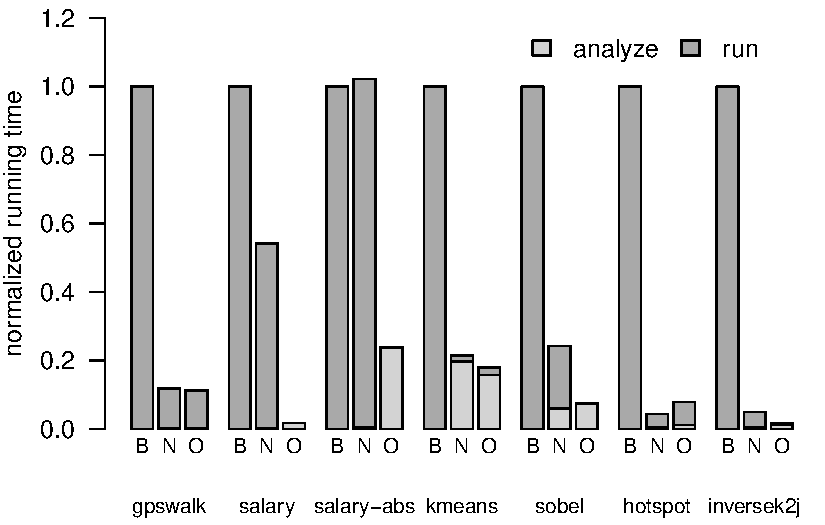
\includegraphics[width=9.5cm]{results/performance}
    \vspace{-1ex}
    \caption{\tool reduces testing time.  We normalize to B: the baseline
      stress-testing technique with 74147 samples. N is \tool without 
      optimizations and O is \tool with optimizations, divided into
      analysis and execution time. Times are averaged over 5 executions.
      We elide error bars as they are very small.}
    \label{passert:fig:performance}
\end{figure}

For most benchmarks, \tool's time is almost exclusively spent on distribution
extraction and optimization, which means optimizations are effective at
producing a very small distribution that can be sampled much more efficiently
than the original program.
The exception is \bench{gpswalk}, where the analysis executed in
\perfdata{time-gpswalk-sample-analyze} seconds
but sampling the resulting distribution took over a minute.
That program's probability distribution consists of thousands of independent
Rayleigh distributions, each with a different parameter as reported by the GPS
sensor, so it cannot take advantage of optimizations that exploit many
samples from identical distributions.

\paragraph{Effect of Optimizations}
We evaluated a variant of \tool with optimizations disabled. This
version simply performs distribution extraction and samples the
resulting distribution.  The middle bars labeled N in
Figure~\ref{passert:fig:performance} show the normalized running time of this
non-optimizing \tool variant.

The effectiveness of the optimizations varies among the benchmarks.
On one extreme, optimizations
reduce the execution time for \bench{salary} from
\perfdata{time-salary-noopt-run} seconds to a fraction of a second.
The unoptimized Bayesian network for \bench{salary-abs} is slightly
\emph{less} efficient than the original program.  The Central Limit
Theorem optimization applies to both and greatly reduces the amount of
sampled computation.  On the other hand, simply evaluating the
extracted distribution delivers a benefit for \bench{gpswalk},
reducing \perfdata{time-gpswalk-dummy-run} to
\perfdata{time-gpswalk-noopt-run} seconds and then optimizations
further reduce this time to just \perfdata{time-gpswalk-sample-run}
seconds.
In a more extreme case, enabling optimizations adds to the analysis time for
\bench{hotspot} but fails to reduce its sampling time.
These programs benefit from eliminating the deterministic
computations involved in timestamp parsing and distance calculation.

\paragraph{Confidence--Performance Trade-off}

Via the confidence and accuracy parameters $\alpha$ and $\epsilon$, \tool
provides rough estimates quickly or more accurate evaluations
using more samples.
% When using fewer samples, the benefits of optimization can be outweighed by
% their costs and the programmer is better off with a brute-force stress-testing
% approach.
To evaluate this trade-off, we lowered the
parameter settings, $\alpha = 0.10$ and $\epsilon = 0.05$, which leads to 2457
samples (about 3\% compared to the more accurate settings above).
Even accounting for analysis time, \tool yields a harmonic mean
\perfdata{o-speedup-harmmean-lowc}
speedup over the baseline in this relaxed configuration.
